% Этот шаблон документа разработан в 2014 году
% Данилом Фёдоровых (danil@fedorovykh.ru) 
% для использования в курсе 
% <<Документы и презентации в \LaTeX>>, записанном НИУ ВШЭ
% для Coursera.org: http://coursera.org/course/latex .
% Исходная версия шаблона --- 
% https://www.writelatex.com/coursera/latex/5.1

%\documentclass[t]{beamer}  % [t], [c], или [b] --- вертикальное выравнивание на слайдах (верх, центр, низ)
\documentclass[c, handout]{beamer} % Раздаточный материал (на слайдах всё сразу)
%\documentclass[aspectratio=169]{beamer} % Соотношение сторон

%\usetheme{Berkeley} % Тема оформления
%\usetheme{Bergen}
%\usetheme{Szeged}

%\usecolortheme{beaver} % Цветовая схема
%\useinnertheme{circles}
%\useinnertheme{rectangles}

\usetheme{Boadilla}
\usecolortheme{dolphin}

%%% Работа с русским языком
\usepackage{cmap}					% поиск в PDF
\usepackage{mathtext} 				% русские буквы в формулах
\usepackage[T2A]{fontenc}			% кодировка
\usepackage[utf8]{inputenc}			% кодировка исходного текста
\usepackage[english,russian]{babel}	% локализация и переносы

%%% Дополнительная работа с математикой
\usepackage{amsmath,amsfonts,amssymb,amsthm,mathtools} % AMS
\usepackage{icomma} % "Умная" запятая: $0,2$ --- число, $0, 2$ --- перечисление

%% Номера формул
%\mathtoolsset{showonlyrefs=true} % Показывать номера только у тех формул, на которые есть \eqref{} в тексте.
%\usepackage{leqno} % Нумерация формул слева

%% Свои команды
\DeclareMathOperator{\sgn}{\mathop{sgn}}
\DeclareMathOperator{\cov}{Cov}
\let\P\relax
\DeclareMathOperator{\P}{\mathbb{P}}
\DeclareMathOperator{\E}{\mathbb{E}}
\DeclareMathOperator{\Var}{Var}

%% Перенос знаков в формулах (по Львовскому)
\newcommand*{\hm}[1]{#1\nobreak\discretionary{}
	{\hbox{$\mathsurround=0pt #1$}}{}}

%%% Работа с картинками
\usepackage{graphicx}  % Для вставки рисунков
\graphicspath{{images/}{images2/}}  % папки с картинками
\setlength\fboxsep{3pt} % Отступ рамки \fbox{} от рисунка
\setlength\fboxrule{1pt} % Толщина линий рамки \fbox{}
\usepackage{wrapfig} % Обтекание рисунков текстом

%%% Работа с таблицами
\usepackage{array,tabularx,tabulary,booktabs} % Дополнительная работа с таблицами
\usepackage{longtable}  % Длинные таблицы
\usepackage{multirow} % Слияние строк в таблице

%%% Программирование
\usepackage{etoolbox} % логические операторы

%%% Другие пакеты
\usepackage{lastpage} % Узнать, сколько всего страниц в документе.
\usepackage{soul} % Модификаторы начертания
\usepackage{csquotes} % Еще инструменты для ссылок
%\usepackage[style=authoryear,maxcitenames=2,backend=biber,sorting=nty]{biblatex}
\usepackage{multicol} % Несколько колонок

%%% Картинки
\usepackage{tikz} % Работа с графикой
\usepackage{pgfplots}
\usepackage{pgfplotstable}

\DeclareMathOperator{\Lin}{\mathrm{Lin}}
\DeclareMathOperator{\Linp}{\Lin^{\perp}}
\DeclareMathOperator*\plim{plim}
%\DeclareMathOperator{\grad}{grad}
\DeclareMathOperator{\card}{card}
%\DeclareMathOperator{\sgn}{sign}
\DeclareMathOperator{\sign}{sign}

\DeclareMathOperator*{\argmin}{arg\,min}
\DeclareMathOperator*{\argmax}{arg\,max}
\DeclareMathOperator*{\amn}{arg\,min}
\DeclareMathOperator*{\amx}{arg\,max}
%\DeclareMathOperator{\cov}{Cov}
%\DeclareMathOperator{\Var}{Var}
\DeclareMathOperator{\Cov}{Cov}
\DeclareMathOperator{\Corr}{Corr}
\DeclareMathOperator{\pCorr}{pCorr}

\let\P\relax
\DeclareMathOperator{\P}{\mathbb{P}}



\newcommand{\cN}{\mathcal{N}}
\newcommand{\cU}{\mathcal{U}}
\newcommand{\cBinom}{\mathcal{Binom}}
\newcommand{\cPois}{\mathcal{Pois}}
\newcommand{\cBeta}{\mathcal{Beta}}
\newcommand{\cGamma}{\mathcal{Gamma}}

\def \R{\mathbb{R}}
\def \N{\mathbb{N}}
\def \Z{\mathbb{Z}}

\title[Введение в ML]{Введение в машинное обучение}
%\subtitle{Monetary Policy in Terms of Capital Outflow}
\author[Омелюсик В.С.]{Омелюсик Владимир Степанович}
\date{23 ноября 2019 г.}
\institute[НИУ ВШЭ]{Национальный Исследовательский Университет \\ <<Высшая школа экономики>> \\ -- \\ Факультатив «Введение в анализ данных и машинное обучение на Python»}

\newcommand{\art}[1]{({\small\textit{#1}})}

\usepackage{hyperref}
\hypersetup{urlcolor=blue,  colorlinks=true, linkcolor=black}

\usepackage{listings}    


\lstset{ 
	language=R,                     % the language of the code
	basicstyle= \ttfamily, % the size of the fonts that are used for the code
	%numbers=left,                   % where to put the line-numbers
	%numberstyle=\tiny\color{blue},  % the style that is used for the line-numbers
	%stepnumber=1,                   % the step between two line-numbers. If it is 1, each line
	% will be numbered
	%numbersep=5pt,                  % how far the line-numbers are from the code
	backgroundcolor=\color{white},  % choose the background color. You must add \usepackage{color}
	showspaces=false,               % show spaces adding particular underscores
	showstringspaces=false,         % underline spaces within strings
	showtabs=false,                 % show tabs within strings adding particular underscores
	%frame=single,                   % adds a frame around the code
	%rulecolor=\color{teal},        % if not set, the frame-color may be changed on line-breaks within not-black text (e.g. commens (green here))
	tabsize=1,                      % sets default tabsize to 2 spaces
	captionpos=b,                   % sets the caption-position to bottom
	breaklines=true,                % sets automatic line breaking
	breakatwhitespace=false,        % sets if automatic breaks should only happen at whitespace
	keywordstyle=\color{black},      % keyword style
	commentstyle=\color{purple},   % comment style
	stringstyle=\color{violet}      % string literal style
} 


\begin{document}
	
	\frame[plain]{\titlepage}	% Титульный слайд
	
	\begin{frame}{Немного истории}
		\begin{itemize}\setlength\itemsep{1em}
			\item<1-> 1956 год – первый семинар по проблемам искусственного интеллекта.
			
			Задача: моделирование интеллекта человека математическими методами.
			
			\item<1-> До 1970-х годов – простейшие системы AI.
			\begin{itemize}
				\item Доказательство теорем методом дедукции.
				\item ELIZA – синтаксический анализатор.
			\end{itemize}
		
			\item<2-> 1980-е годы – решающие деревья.
			
			В каждом узле дерева стоит некоторое условие. В зависимости от выполнения данного условия, дерево переходит в следующую ветвь. 
		\end{itemize}
	\end{frame}

	\begin{frame}{Дерево решений: пример}
		\begin{center}
		\frame{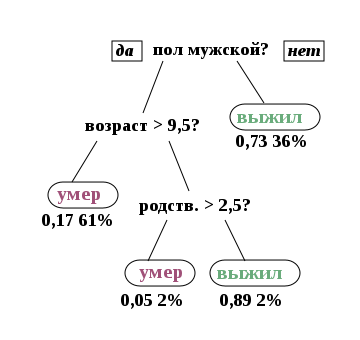
\includegraphics[width=0.5\linewidth]{tit.png}}\\
		{\tiny Задача «Титаник» (\href{https://ru.wikipedia.org/wiki/Дерево_решений}{Источник})}
		\end{center}
	\end{frame}

	\begin{frame}{Немного истории}
		\begin{itemize}\setlength\itemsep{1em}
			\item 1990-е годы – развитие более продвинутых систем машинного обучения:
			\begin{itemize}
				\item Нейронные сети.
				\item Генетические алгоритмы.
			\end{itemize}
			\item 2000-е годы и современность – Deep Learning.
			
			Построение моделей с очень высокой точностью распознавания.
		\end{itemize}
	\end{frame}
	
	\begin{frame}{Определение}
		\begin{block}{Машинное обучение}
			Область науки, изучающая построение моделей и алгоритмов, позволяющих компьютерным системам воспроизводить \alert{зависимости} между различными объектами \alert{без} их непосредственного \alert{программирования}. 
		\end{block}\vspace{1em}
	
	Неформально:
		\begin{itemize}
			\item «Обучение» специальных моделей на некоторых данных.
			\item  В ходе «обучения» происходит «запоминание» зависимостей, представленных в данных (важна репрезентативность выборки). 
			\item После «обучения» модель способна давать корректные предсказания на новых данных.
		\end{itemize}
	
	\end{frame}

	\begin{frame}{Зависимости}
		\begin{itemize}\setlength\itemsep{1em}
			\item<1-> Зависимости позволяют нам давать ответы на интересующие нас вопросы.
			\item<1-> Зависимость можно сформулировать словесно:
				\begin{itemize}\setlength\itemsep{0.4em}
					\item «Площадь прямоугольника равна произведению его длины и ширины». 
					\item «Вероятность выжить на Титанике зависит от пола пассажира».
					\item «Вероятность того, что данный цветок ириса принадлежит к виду I. kaempferi, зависит от длины его лепестков».
				\end{itemize}
			\item<2-> Но для получения чётких количественных результатов нужно формализовать словесные формулировки.
			\item<2-> Необходимо выразить их математическими функциями. 
			\item<2-> Это не всегда просто (иногда – невозможно), так как истинные функции могут быть достаточно сложными. 
		\end{itemize}
		
	\end{frame}

	\begin{frame}{Пример зависимости: килограммы и тонны}
		\begin{itemize}
			\item<1-> Вопрос: как перевести массу в тоннах в массу в килограммах?
			\item<2-> Зависимость: 1 тонна = 1000 кг.
			\item<2-> Формализация:
			\[
			f(x) = \dfrac{x}{1000},
			\] 
			где $x$ – масса в тоннах.
		\end{itemize}
	\end{frame}

	\begin{frame}{Пример зависимости: предсказание погоды}
		
		\begin{itemize}
			
		\item<1-> Вопрос: какая завтра будет погода? 
		
		\item<2-> Зависимость: как погода завтра зависит от $\ldots$?
		
		\item<3-> Формализация:
		
		Уравнения Навье-Стокса (частично, \href{https://latex.org/forum/viewtopic.php?t=22487}{источник}):
		
		\begin{equation}
		\frac{\partial \rho}{\partial t} + \overrightarrow{\nabla}\cdot(\rho\overrightarrow{u})=0 \end{equation}
		\begin{equation}
		\frac{\partial(\rho \overrightarrow{u})}{\partial t} + \overrightarrow{\nabla}\cdot[\rho\overline{\overline{u\otimes u}}] = -\overrightarrow{\nabla p} + \overrightarrow{\nabla}\cdot\overline{\overline{\tau}} + \rho\overrightarrow{f} \end{equation}
		\begin{equation}
		\frac{\partial(\rho e)}{\partial t} + \overrightarrow{\nabla}\cdot((\rho e + p)\overrightarrow{u}) = \overrightarrow{\nabla}\cdot(\overline{\overline{\tau}}\cdot\overrightarrow{u}) + \rho\overrightarrow{f}\overrightarrow{u} + \overrightarrow{\nabla}\cdot(\overrightarrow{\dot{q}})+r \end{equation}
		
		\item<3-> Позволяют найти давление и скорость воздуха в любой точке. Но тяжело решать. 
		\end{itemize}
		
	\end{frame}

	\begin{frame}{Пример зависимости: анализ тональности текста}
		\begin{center}
			«Быть или не быть, вот в чем вопрос. Достойно ль \\
			Смиряться под ударами судьбы...»
		\end{center}
		\begin{flushright}
			{\small У. Шекспир «Гамлет»}
		\end{flushright}
	\begin{itemize}
		\item<1-> Вопрос: какая тональность у данного фрагмента текста?
		\item<2-> Зависимость: $\ldots$?
		\item<2-> Формализация: $x$ – фрагмент текста, $f(x) = \ldots$? Непонятно.
		
	\end{itemize}

	\end{frame}

	
	\begin{frame}{Более сложные вопросы}
		
		\begin{itemize}
			\item Какой будет спрос на овощи в продуктовом магазине в следующем месяце?
			\item Выдать ли клиенту кредит? 
			\item На фотографии кошка или собака? 
		\end{itemize}
	
		Найти точные математические функции для ответа на данные вопросы сложно (или невозможно). Но если у нас есть некоторый набор данных, можно попытаться \alert{приблизить} зависимости некоторыми математическими моделями.
	\end{frame}
		
	\begin{frame}{Приближение зависимостей}
		\begin{block}{Цель машинного обучения}
			Используя только данные, а не теорию, попытаться восстановить истинные зависимости.
		\end{block}
		
		\begin{itemize}
			\item<1-> Пример с монеткой: истинная вероятность того, что выпадет орёл равна $p$, её оценка равна $\hat{p}$.
			\item<2-> Формально: пусть истинная зависимость: $y(x)$ – и её мы не знаем. Будем пытаться по данным подобрать некоторую функцию $\hat{y}(x)$, которая приближает истинную зависимость. 
		\end{itemize}	
	\end{frame}
			
	\begin{frame}{Применение машинного обучения: AlphaGo}
		 \begin{itemize}
		 	\item Нейронная сеть, победившая чемпиона мира в 2016 году.
		 	\item Обучалась, играя сама с собой.
		 \end{itemize}
	 \begin{center}
	 	\href{https://www.cbsnews.com/news/human-champ-stunned-as-computer-wins-at-go/}{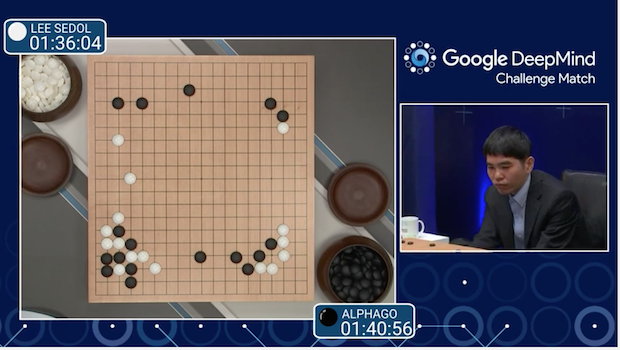
\includegraphics[width=\linewidth]{go.png}} \\	 		
	 \end{center}
 	\end{frame}
 
 	\begin{frame}{Применение машинного обучения: ImageNet}
 		\begin{itemize}
 			\item Соревнование по распознаванию объектов на изображении.
 			\item Решается с помощью нейронных сетей.
 		\end{itemize}
 	 \begin{center}
 		\href{http://www.image-net.org/challenges/LSVRC/2014/}{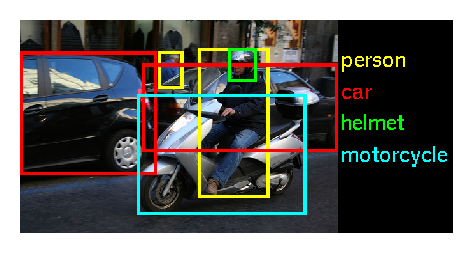
\includegraphics[width=\linewidth]{in.png}}
 	\end{center}
 	\end{frame}
 
 	\begin{frame}{Применение машинного обучения: Отдел кадров}
 		\begin{itemize}
 			\item Поиск кандидатов, предсказание результата собеседования.
 			\item Предсказание ухода сотрудника.
 			\item Анализ внутренних каналов информации, определение жалоб.
 		\end{itemize}
 	\end{frame}
	
	\begin{frame}{Применение машинного обучения: Рекомендательные и поисковые системы}
		\begin{itemize}
			\item Рекомендательные системы: Netflix, Amazon, $\ldots$ – на основании поведения пользователя определяют, какой товар или услугу разумно ему предложить. 
			\item Поисковые системы: Google, Яндекс, $\ldots$ – на основании запроса пользователя определяют, какие веб-сайты наиболее соответствуют запросу.  
		\end{itemize}		
	\end{frame}

	\begin{frame}{Применение машинного обучения: Чтение по губам}
		\begin{itemize}
			\item Google Deepmind: модель, которая была способна превзойти профессионального чтеца по губам.
		\end{itemize}
		\begin{center}
			\href{https://www.newscientist.com/article/2113299-googles-deepmind-ai-can-lip-read-tv-shows-better-than-a-pro/}{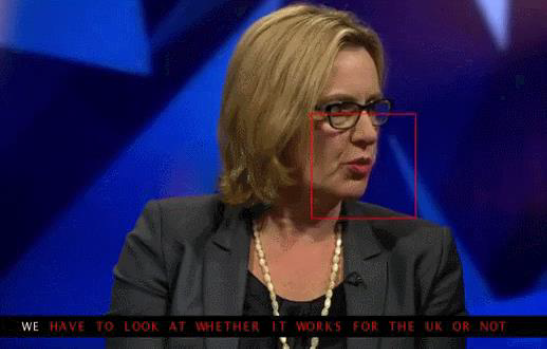
\includegraphics[width=0.9\linewidth]{dm.png}}
		\end{center}
	\end{frame}

	\begin{frame}{Типы задач машинного обучения}
		\begin{itemize}
			\item<1-> Мы уже знакомы с основными понятиями машинного обучения: целевая переменная (target) и признаки (features).
			\item<2-> Типы задач машинного обучения (в зависимости от наличия целевой переменной):
			\begin{enumerate}
				\item Обучение с учителем (supervised learning).
					\begin{itemize}
						\item \alert{Классификация}.
						\item \alert{Регрессия}.
						\item Ранжирование.
					\end{itemize}
				\item Обучение без учителя (unsupervised learning).
					\begin{itemize}
						\item \alert{Кластеризация}.
					\end{itemize}
				\item Обучение с подкреплением (reinforcement learning).
			\end{enumerate}
		\end{itemize}
	\end{frame}

	\begin{frame}{Обучение с учителем}
		\begin{block}{Обучение с учителем}
			Вид обучения, когда имеется целевая переменная, и модель обучается так, чтобы наиболее правильно предсказывать целевую переменную.  
		\end{block}
	\vspace{0.7cm}
	В обучении с учителем выделяют следующие виды задач:
	\begin{itemize}
		\item Регрессия: $Y \in \R$.
		\item Классификация: $|Y| < \infty$.
		\item Ранжирование: $Y$ – конечное упорядоченное множество.
 	\end{itemize}
	\end{frame}

	\begin{frame}{Задача регрессии}
		\begin{itemize}
			\item<1-> $Y \in \R$, то есть зависимая переменная может принимать любые вещественные значения (бесконечное число значений).
			\item<2-> Пример: линейная регрессия
			\[
			\hat{Y}_i = \hat{\beta}_0 + \hat{\beta}_1X_{1i} + \hat{\beta}_2X_{2i} + \ldots \hat{\beta}_kX_{ki},
			\]
			где $\hat{\beta}_0$, $\hat{\beta}_1$, $\ldots$, $\hat{\beta}_k$ – оценки истинных коэффициентов.
		\end{itemize}
	\end{frame}
	
	\begin{frame}{Задача регрессии: Пример}
		
		Предсказание цены на жильё в зависимости о среднего числа комнат (по датасету {\tt boston} в {\tt sklearn}):
		
		\[
		\hat{Y}_i = -34.67 + 9.1X^{RM}_i 
		\]
		
		\begin{center}
			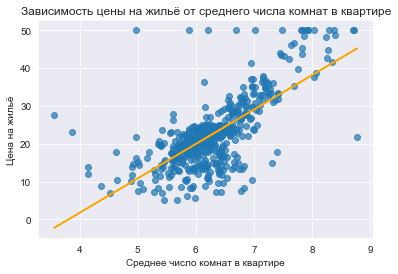
\includegraphics[width=0.7\linewidth]{b.png}
		\end{center}
	
	\end{frame}

	\begin{frame}{Задача классификации}
		\begin{itemize}
			\item<1-> $|Y| < \infty$, то есть зависимая переменная может принимать ограниченное число значений.
			\item<2-> Виды:
			\begin{itemize}
				\item Бинарная классификация: $Y = 1$ или $Y = 0$.
				\item Многоклассовая классификация: $Y = 1$, или $Y = 2$, $\ldots$, или $Y = K$.
				\item Классификация с пересекающимися классами: $Y$ может принимать несколько значений из множества: $\{1, 2, \ldots K\}$.
			\end{itemize}
		\end{itemize}
		
	\end{frame}

	\begin{frame}{Бинарная классификация: Пример}
		Задача: провести линию так, чтобы наиболее точно разделить объекты разных классов.
		
		\begin{center}
			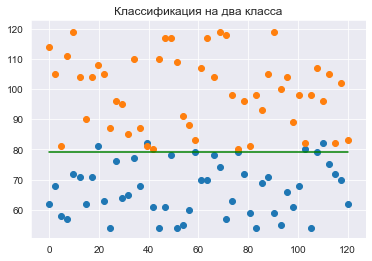
\includegraphics[width=0.6\linewidth]{c.png}
		\end{center}
	\end{frame}

	\begin{frame}{Многоклассовая классификация: Пример}
		Задача: провести линии так, чтобы наиболее точно разделить объекты разных классов.
		
		\begin{center}
			\href{https://scikit-learn.org/stable/modules/multiclass.html}{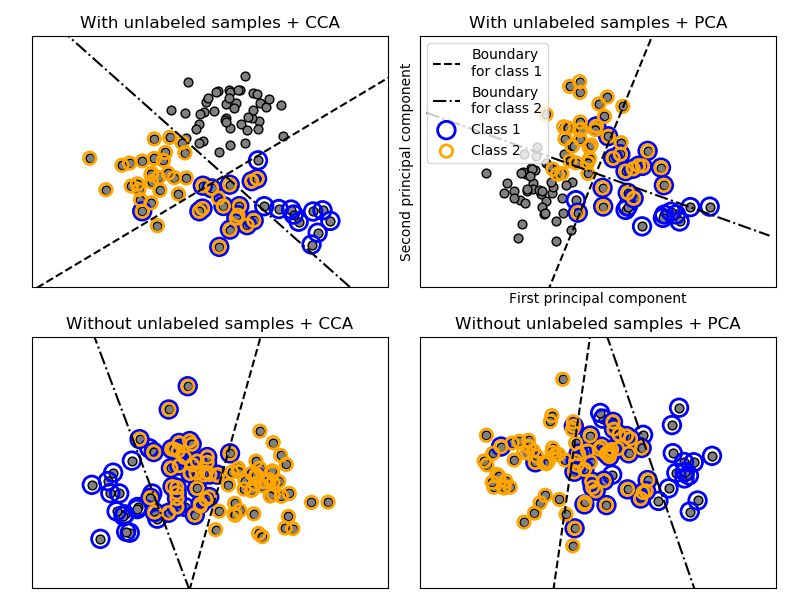
\includegraphics[width=0.7\linewidth]{mlc.png}}
		\end{center}
	\end{frame}

	\begin{frame}{Примеры реальных задач классификации и регрессии}
		\begin{enumerate}
			\item<1-> Медицинская диагностика.
			\begin{itemize}
				\item Наблюдение: пациент в момент времени $t$.
				\item Предсказание: диагноз.
			\end{itemize}
			\item<2-> Предсказание оттока клиентов.
			\begin{itemize}
				\item Наблюдение: клиент в момент времени $t$.
				\item Предсказание: уйдёт или нет в течение трёх месяцев.
			\end{itemize}
			\item<3-> Прогнозирование времени сна млекопитающих.
			\begin{itemize}
				\item Наблюдение: млекопитающее в момент времени $t$.
				\item Предсказание: среднее время сна в сутки в секундах.
			\end{itemize}
		\end{enumerate}
	\end{frame}

	\begin{frame}{Примеры реальных задач классификации и регрессии}
		\begin{enumerate}
			\item Медицинская диагностика.
			\begin{itemize}
				\item Наблюдение: пациент в момент времени $t$.
				\item Предсказание: диагноз.
				\item Многоклассовая классификация.
			\end{itemize}
			\item Предсказание оттока клиентов.
			\begin{itemize}
				\item Наблюдение: клиент в момент времени $t$.
				\item Предсказание: уйдёт или нет в течение трёх месяцев.
				\item Бинарная классификация.
			\end{itemize}
			\item Прогнозирование времени сна млекопитающих.
			 \begin{itemize}
			 	\item Наблюдение: млекопитающее в момент времени $t$.
			 	\item Предсказание: среднее время сна в сутки в секундах.
			 	\item Регрессия.
			 \end{itemize}
		\end{enumerate}
	\end{frame}

	\begin{frame}{Задача ранжирования}
		\begin{itemize}
			\item $Y$ – конечное упорядоченное множество (например, пользовательские оценки веб-сайтов).
			\item Дан набор «запросов» $Q = (q_1, q_2, \ldots q_n)$ и набор «документов» $D = (d_1, d_2, \ldots d_m)$.
			\item Цель: используя $Y$, построить модель $R(q_i, D)$, которая для запроса $q$ «правильно» бы упорядочивала набор документов $D$.
		\end{itemize}
		
	\end{frame}

	\begin{frame}{Задача ранжирования: Пример}
		Задача: упорядочить веб-сайты в соответствии с релевантностью запросу.
		
		\begin{center}
			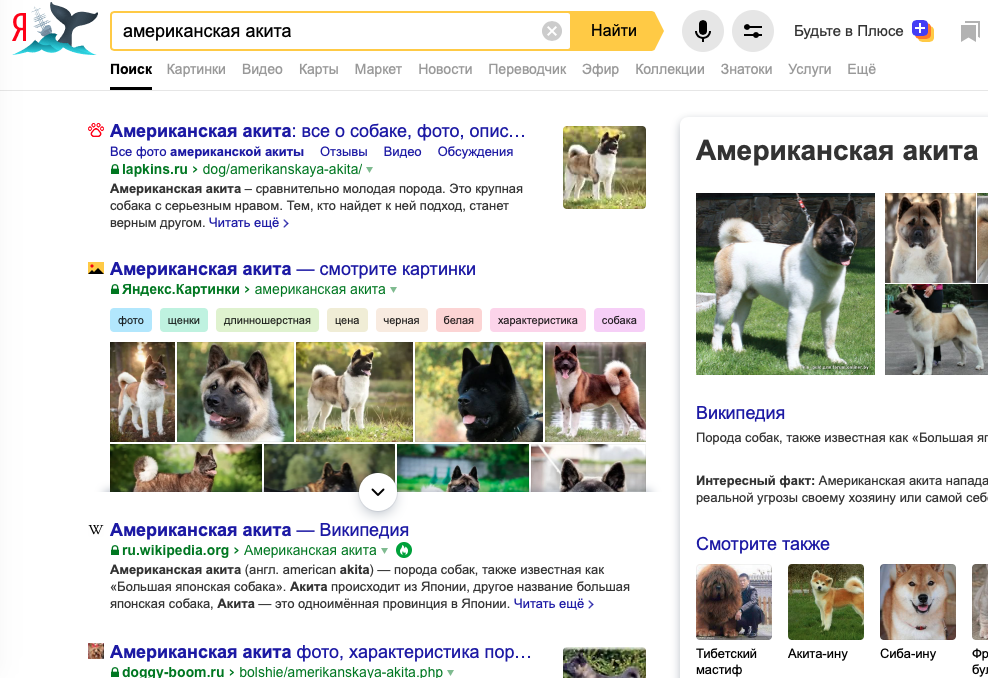
\includegraphics[width=0.8\linewidth]{r.png}
		\end{center}
	\end{frame}

	\begin{frame}{Обучение без учителя}
		\begin{block}{Обучение без учителя}
			Вид обучения, когда целевая переменная неизвестна или отсутствует, и модель обучается только по признакам объектов.  
		\end{block}
	\begin{itemize}
		\item Задача кластеризации: $Y$ – отсутствует. \\
		\vspace{1em}
		Цель: найти группы похожих объектов (то есть разделить выборку на кластеры). \\
		\vspace{1em}
		Обучение происходит только на основе признаков объектов.
	\end{itemize}
	\end{frame}

\begin{frame}{Задача кластеризации: Пример}
	Задача: разбить представленную выборку на кластеры, руководствуясь только признаковым описанием объектов.
	
	\begin{center}
		\href{https://en.wikipedia.org/wiki/Cluster_analysis}{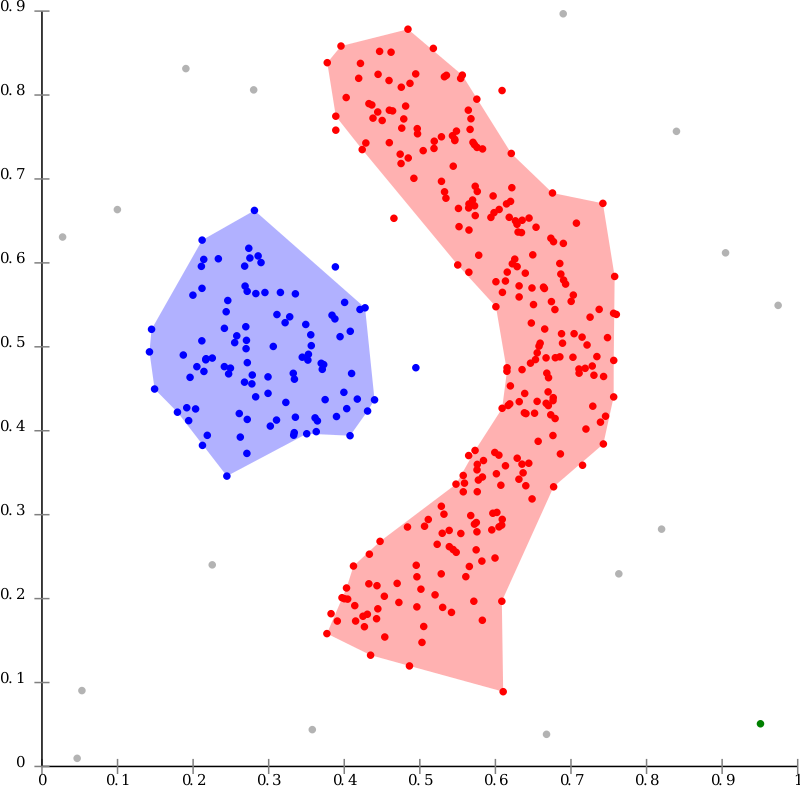
\includegraphics[width=0.5\linewidth]{cl.png}}
	\end{center}
\end{frame}

\begin{frame}{Обучение с подкреплением}
	
	\begin{itemize}
		\item<1-> Другой подход к обучению: существует \textit{среда} и отделённый от неё \textit{агент}.
		\item<1-> На каждом шаге агент получает вознаграждение за выполненное им действие (может быть отрицательным).
		\item<1-> Учитель отсутствует: обучение происходит через максимизацию суммарного вознаграждения. 
		\item<2-> Примеры:
		\begin{itemize}
			\item AlphaGo.
			\item Контроль движений робота.
			\item Управление энергетической станцией.
			\item Реализация управления вертолётом.
		\end{itemize}
	\end{itemize}
\end{frame}

\begin{frame}{Обучение с подкреплением: Пример}
	Задача: научить агента использовать нужные движения, чтобы переместиться на максимальное расстояние.
	
	\begin{center}
		\href{https://towardsdatascience.com/training-a-cheetah-to-run-with-deep-reinforcement-learning-6dca2975443a?gi=3ca7d8cbbbdd}{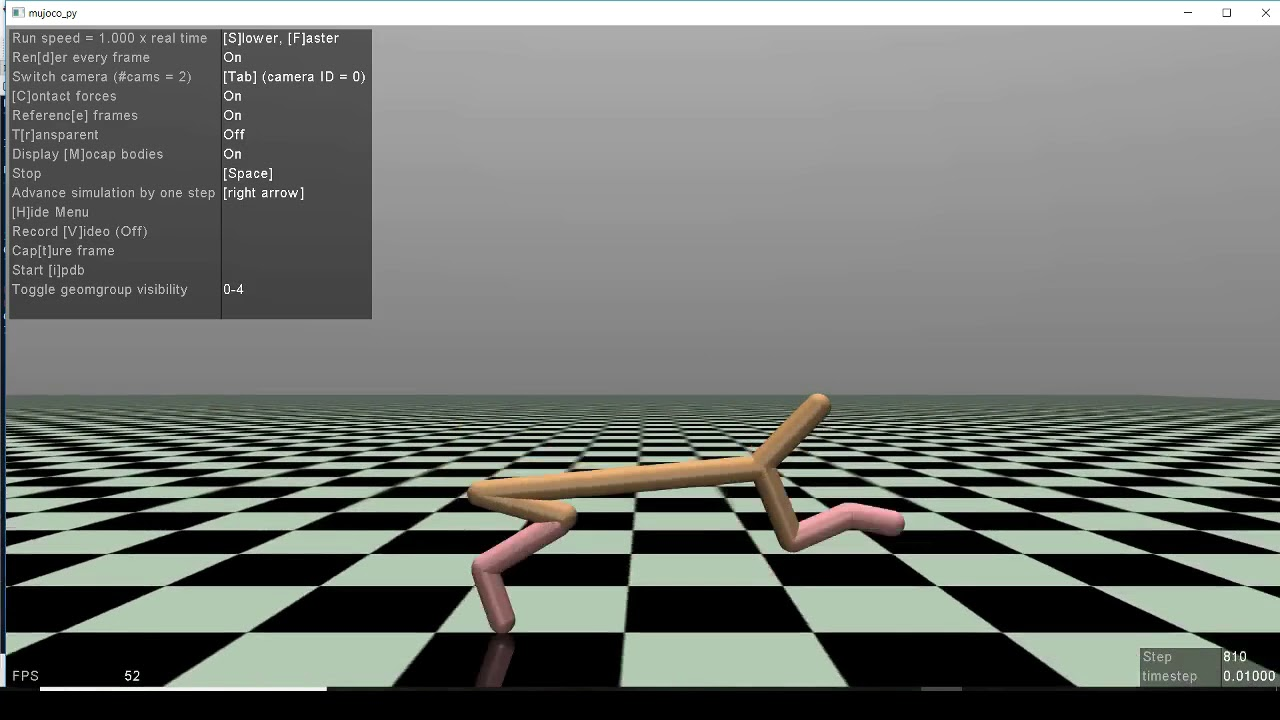
\includegraphics[width=0.9\linewidth]{hc.jpg}}
	\end{center}
\end{frame}

\begin{frame}{Другие понятия машинного обучения}
	\begin{itemize}\setlength\itemsep{1em}
		\item<1-> Что знаем теперь:
		\begin{itemize}
			\item Можем решать разные типы задач: регрессия, классификация, кластеризация. 
			\item $Y$ – зависимая переменная, $X_1$, $X_2$, $\ldots$ – признаки.
			\item Хотим восстановить зависимость $Y(X)$ (для обучения с учителем).
			\item Для восстановления зависимости строим модель $\hat{Y}(X)$.
		\end{itemize}
		\item<2-> Как происходит обучение? $\Rightarrow$ Функция потерь.
		\item<2-> Как определить качество модели? $\Rightarrow$ Функционал качества, Обобщающая способность.
	\end{itemize}
\end{frame}

\begin{frame}{Функция потерь}
	\begin{block}{Функция потерь}
		Функция, измеряющая ошибку алгоритма. Иначе говоря, мера корректности алгоритма. 
	\end{block}
	\begin{itemize}
		\item Много различных вариантов.
		\item Алгоритм \alert{обучается путём минимизации функции потерь}. 
		\item Пример: среднеквадратичная ошибка (MSE, mean squared error):
		\[
		\dfrac{1}{n} \sum_{i=1}^{n}\left( Y_i - \hat{Y}_i  \right)^2 
		\]
	\end{itemize}
\end{frame}

\begin{frame}{Функционал (метрика) качества}
	\begin{block}{Функционал качества}
		Функция, используемая для оценки качества и сравнения различных моделей.
	\end{block}
	\begin{itemize}
		\item Много различных вариантов.
		\item С помощью функционала качества \alert{мы сравниваем различные модели}. 
		\item Пример: доля правильных ответов (accuracy) – для задачи классификации:
		\[
		\dfrac{1}{n}\sum_{i=1}^{n}\mathbb{I}\{\hat{Y}_i = Y_i\},
		\]
		где $\mathbb{I}\{\cdot\} = \begin{cases}
		1, \text{ если условие в скобках выполнено.} \\
		0, \text{ если условие в скобках не выполнено.}
		\end{cases}$
	\end{itemize}
\end{frame}

\begin{frame}{Обобщающая способность}
	\begin{block}{Обобщающая способность}
		Способность модели давать корректные предсказания на новых данных, не участвовавших при её обучении. 
	\end{block}
	
	\begin{block}{Недообучение}
		Ситуация, когда модели не удалось правильно «запомнить» зависимости в данных. В этом случае качество будет \alert{низким как на обучающей выборке, так и на новых данных}.
	\end{block}

	\begin{block}{Переобучение}
	Ситуация, когда модель идеально «запомнила» соотношения, представленные в обучающей выборке, но не зависимости в данных. В этом случае качество будет \alert{высоким на обучающей выборке, но низким на новых данных}.
	\end{block}
\end{frame}

\begin{frame}{Обобщающая способность}
	\begin{itemize}
		\item<1-> В случаях недо- и переобучения обобщающая способность модели низкая.
		\item<1-> Пример: синий – истинная зависимость, оранжевый – оценённая зависимость, фиолетовый – выборка.
	\end{itemize}
	\begin{center}
	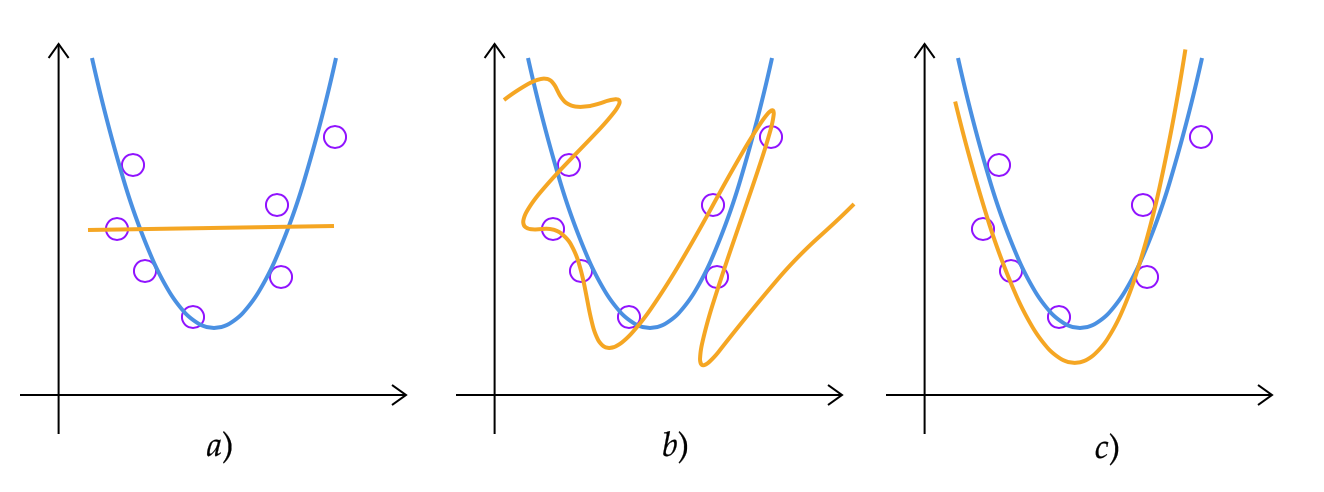
\includegraphics[width=0.9\linewidth]{f.png}
	\end{center}
	\begin{itemize}
		\item<2-> $a)$ – недообучение, $b)$ – переобучение, $c)$ – корректно обученная модель.
	\end{itemize}
\end{frame}


\end{document}